\subsection*{1.4 System of Two Linear Equations In Two Variables }
\vspace{0.5em}

\setcounter{questionnum}{0}

\noindent\markforreview

\vspace{0.5em}
\[
\begin{aligned}
-x + y = -3.5 \\ 
x + 3y = 9.5
\end{aligned}
  \]


If $(x, y)$ satisfies the system of equations above, what is the value of $y$?


\vspace{5em}
\noindent\markforreview

\vspace{0.5em}

\[
\begin{aligned}
\frac{3}{2}y - \frac{1}{4}x &= \frac{2}{3}-\frac{3}{2}y \\
\frac{1}{2}x + \frac{3}{2} &= py + \frac{9}{2}
\end{aligned}
\]

In the given system of equations, $p$ is a constant. If the system has no solution, what is the value of $p$?


\vspace{5em}
\noindent\markforreview

\vspace{0.5em}

\[
\begin{aligned}
4x - 6y &= 10y + 2 \\
ty &= \frac{1}{2} + 2x
\end{aligned}
\]

In the given system of equations, $t$ is a constant. If the system has no solution, what is the value of $t$?

\newpage
\noindent\markforreview

\vspace{1em}

During a month, Morgan ran $r$ miles at 5 miles per hour and biked $b$ miles at 10 miles per hour. She ran and biked a total of 200 miles that month, and she biked for twice as many hours as she ran. What is the total number of miles that Morgan biked during the month?

\vspace{0.75em}

\choicebox{A}{80}
\choicebox{B}{100}
\choicebox{C}{120}
\choicebox{D}{160}


\vspace{2em}
\noindent\markforreview

\vspace{1em}

In the system of equations below, \( a \) and \( c \) are constants.
\[
\frac{1}{2}x + \frac{1}{3}y = \frac{1}{6}
\]
\[
ax + y = c
\]
If the system of equations has an infinite number of solutions \( (x, y) \), what is the value of \( a \)?

\vspace{0.75em}

\choicebox{A}{$-\dfrac{1}{2}$}
\choicebox{B}{$0$}
\choicebox{C}{$\dfrac{1}{2}$}
\choicebox{D}{$\dfrac{3}{2}$}

\newpage
\noindent\markforreview

\vspace{1em}

\[
y = 4x + 1
\]
\[
4y = 15x - 8
\]
The solution to the given system of equations is \( (x, y) \). What is the value of \( x - y \)?

\vspace{5em}



\noindent\markforreview

\vspace{1em}

\[
\begin{aligned}
7x - 5y &= 4 \\
4x - 8y &= 9
\end{aligned}
\]
If \( (x, y) \) is the solution to the system of equations above, what is the value of \( 3x + 3y \)?

\vspace{0.75em}

\choicebox{A}{$-13$}
\choicebox{B}{$-5$}
\choicebox{C}{$5$}
\choicebox{D}{$13$}


\newpage

\noindent\markforreview

\vspace{1em}

In the given system of equations, \( r \) is a constant. If the system has no solution, what is the value of \( r \)?

\[
\begin{aligned}
48x - 72y &= 30y + 24 \\
ry &= \frac{1}{6} - 16x
\end{aligned}
\]

\vspace{5em}
\noindent\markforreview

\vspace{1em}

The solution to the given system of equations is \( (x, y) \). What is the value of \( y \)?

\[
\begin{aligned}
24x + y &= 48 \\
6x + y &= 72
\end{aligned}
\]

\vspace{5em}
\noindent\markforreview

\vspace{1em}

A movie theater sells two types of tickets, adult tickets for \$12 and child tickets for \$8. If the theater sold 30 tickets for a total of \$300, how much, in dollars, was spent on adult tickets? (Disregard the \$ sign when gridding your answer.)

\newpage
\noindent\markforreview

\vspace{1em}

The solution to the given system of equations is \( (x, y) \). What is the value of \( xy \)?

\[
\begin{aligned}
5x + 14y &= 45 \\
10x + 7y &= 27
\end{aligned}
\]

\vspace{2em}

\noindent\markforreview

\vspace{1em}

In the system of equations below, \( c \) is a constant. If the system has no solution, what is the value of \( c \)?

\[
\begin{aligned}
y &= \frac{1}{2}x + 8 \\
y &= cx + 10
\end{aligned}
\]

\vspace{2em}

\noindent\markforreview

\vspace{1em}

In the system of equations above, \( a \) is a constant. If the system of equations has no solution, what is the value of \( a \)?

\[
\begin{aligned}
y &= 2x + 1 \\
y &= ax - 8
\end{aligned}
\]

\vspace{0.75em}

\choicebox{A}{$-\dfrac{1}{2}$}
\choicebox{B}{$0$}
\choicebox{C}{$1$}
\choicebox{D}{$2$}

\newpage
\noindent\markforreview

\vspace{1em}

For each real number \( r \), which of the following points lies on the graph of each equation in the \( xy \)-plane for the given system?

\[
\begin{aligned}
8x + 7y &= 9 \\
24x + 21y &= 27
\end{aligned}
\]

\vspace{0.75em}

\choicebox{A}{$(r, -\frac{8r}{7} + \frac{9}{7})$}
\choicebox{B}{$(-\frac{8r}{7} + \frac{9}{7}, r)$}
\choicebox{C}{$(-\frac{8r}{7} + 9, \frac{9r}{7} + 27)$}
\choicebox{D}{$(\frac{r}{3} + 9, -\frac{r}{3} + 27)$}

\vspace{2em}


\noindent\markforreview

\vspace{1em}

Store A sells raspberries for \$5.50 per pint and blackberries for \$3.00 per pint. Store B sells raspberries for \$6.50 per pint and blackberries for \$8.00 per pint. A certain purchase of raspberries and blackberries would cost \$37.00 at Store A or \$66.00 at Store B. How many pints of blackberries are in this purchase?

\vspace{0.75em}

\choicebox{A}{4}
\choicebox{B}{5}
\choicebox{C}{8}
\choicebox{D}{12}



\newpage


\noindent\markforreview

\vspace{1em}

In the given system of equations, \( h \) is a constant. If the system has no solution, what is the value of \( h \)?
\[
\begin{aligned}
4x - 9y &= 9y + 5 \\
hy &= 2 + 4x
\end{aligned}
\]

\vspace{0.75em}

\choicebox{A}{$-9$}
\choicebox{B}{$0$}
\choicebox{C}{$9$}
\choicebox{D}{$18$}

\vspace{2em}
\noindent\markforreview

\vspace{1em}

One of the two equations in a linear system is \( 2x + 6y = 10 \). The system has no solution. Which of the following could be the other equation in the system?

\vspace{0.75em}

\choicebox{A}{$x + 3y = 5$}
\choicebox{B}{$x + 3y = -20$}
\choicebox{C}{$6x - 2y = 0$}
\choicebox{D}{$6x + 2y = 10$}

\newpage
\noindent\markforreview

\vspace{1em}

For each real number \( r \), which of the following points lies on the graph of each equation in the \( xy \)-plane for the given system?
\[
\begin{aligned}
2x + 3y &= 7 \\
10x + 15y &= 35
\end{aligned}
\]

\vspace{0.75em}

\choicebox{A}{$\left(\frac{7}{5} + r, -\frac{7}{5} + 35 \right)$}
\choicebox{B}{$\left(-\frac{3r}{2} + \frac{7}{2}, r \right)$}
\choicebox{C}{$\left(r, \frac{2r}{3} + \frac{7}{3} \right)$}
\choicebox{D}{$\left(r, -\frac{3r}{2} + \frac{7}{2} \right)$}


\vspace{2em}

\noindent\markforreview

\vspace{1em}

One of the equations in a system of two linear equations is given:
\[
y = 6x + 18
\]
The system has no solution. Which equation could be the second equation in the system?

\vspace{0.75em}

\choicebox{A}{$-6x + y = 18$}
\choicebox{B}{$-6x + y = 22$}
\choicebox{C}{$-12x + y = 36$}
\choicebox{D}{$-12x + y = 18$}


\newpage 
\noindent\markforreview

\vspace{1em}

\begin{center}
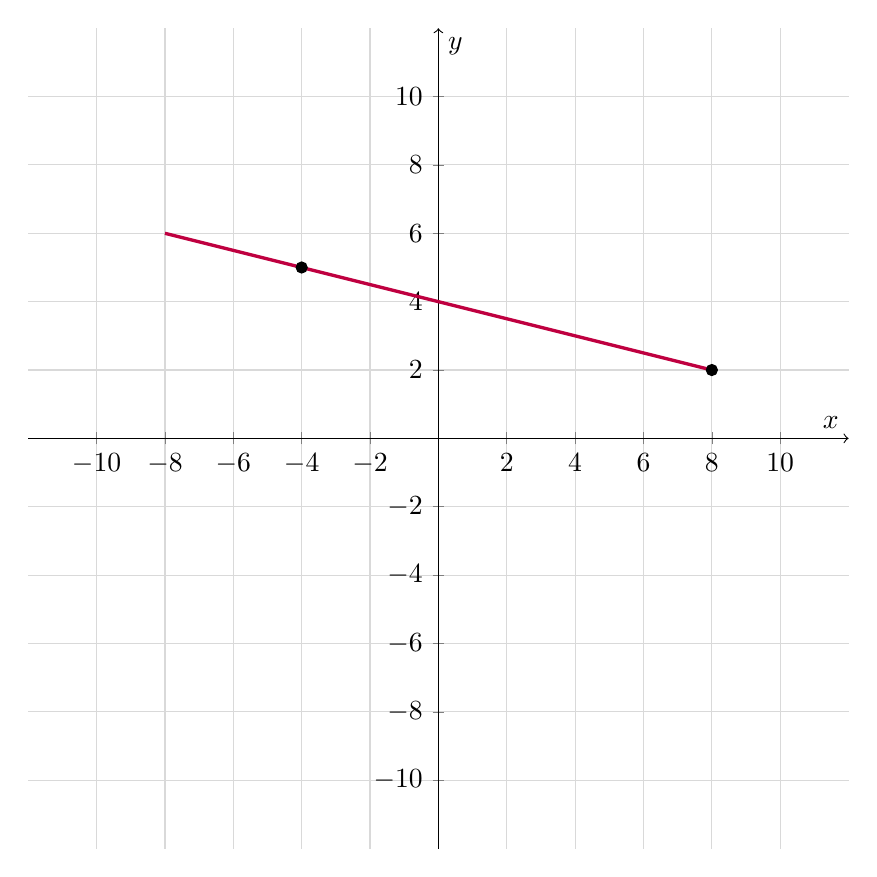
\begin{tikzpicture}[scale=1]
  \begin{axis}[
    axis lines=center,
    xmin=-10, xmax=10,
    ymin=-10, ymax=10,
    xtick={-10,-8,...,10},
    ytick={-10,-8,...,10},
    grid=both,
    width=12cm,
    height=12cm,
    enlargelimits=true,
    xlabel={$x$}, ylabel={$y$},
    ticks=both,
    every major grid/.style={gray!30},
    axis line style={->},
  ]
    % Plot the line
    \addplot[very thick, purple] coordinates {(-8,6) (8,2)};
    \filldraw [black] (-4,5) circle (2pt);
    \filldraw [black] (8,2) circle (2pt);
  \end{axis}
\end{tikzpicture}
\end{center}

If a new graph of three linear equations is created using the system of equations shown and the equation \( x + 4y = -16 \), how many solutions \( (x, y) \) will the resulting system of three equations have?

\vspace{0.75em}

\choicebox{A}{Zero}
\choicebox{B}{Exactly one}
\choicebox{C}{Exactly two}
\choicebox{D}{Infinitely many}


\newpage
